% ============================================================
%  75 % knock-down trebuchet -- laser-cut parts, glue-up, setup
%  6 mm plywood, 900 x 600 bed. Compile with pdflatex (twice)
%  beside out/ and the view_*.pdf files made by views.py
% ============================================================
\documentclass[11pt,a4paper]{article}
\usepackage[T1]{fontenc}
\usepackage[a4paper, top=1.2cm, bottom=1.6cm, left=1.5cm, right=1.5cm]{geometry}
\usepackage{xcolor}
\usepackage{graphicx}
\usepackage{booktabs}
\usepackage{array}
\usepackage{tabularx}
\usepackage{enumitem}
\usepackage{fancyhdr}
\usepackage[protrusion=true,expansion=false]{microtype}

\definecolor{Ink}{HTML}{1A1A1A}
\definecolor{HeadGrey}{HTML}{333333}
\definecolor{RuleGrey}{HTML}{888888}
\definecolor{LineGrey}{HTML}{555555}
\definecolor{WarnBg}{HTML}{F5F5F5}
\definecolor{CutRed}{HTML}{FF0000}
\definecolor{EngBlue}{HTML}{0000FF}

\setlength{\parindent}{0pt}
\setlength{\parskip}{3pt}
\renewcommand{\arraystretch}{1.15}
\newcolumntype{L}[1]{>{\raggedright\arraybackslash}p{#1}}
\newcolumntype{Y}{>{\raggedright\arraybackslash}X}

\newcommand{\sechead}[1]{%
  \par\vspace{5pt}%
  {\bfseries\large\color{HeadGrey} #1}\\[-4pt]
  {\color{RuleGrey}\rule{\linewidth}{0.8pt}}\par\vspace{1pt}}
\newcommand{\warnbox}[1]{%
  \par\vspace{3pt}\noindent
  \fcolorbox{LineGrey}{WarnBg}{\parbox{\dimexpr\linewidth-2\fboxsep-2\fboxrule}{\small #1}}\par\vspace{3pt}}

\pagestyle{fancy}
\fancyhf{}
\renewcommand{\headrulewidth}{0pt}
\fancyfoot[L]{\footnotesize\color{RuleGrey} Trebuchet, 75\,\% knock-down \textbullet{} 4\,kg counterweight \textbullet{} 6\,mm plywood}
\fancyfoot[R]{\footnotesize\color{RuleGrey} Page \thepage}

\begin{document}
\small

{\LARGE\bfseries\color{Ink} Knock-down trebuchet (75\,\%) --- laser-cut parts}\\[3pt]
{\color{RuleGrey}\rule{\linewidth}{1.2pt}}

The 75\,\% oval trebuchet (throwing arm 750\,mm, 4\,kg counterweight), cut from \textbf{four sheets of 6\,mm plywood} on a \textbf{900 $\times$ 600\,mm} bed. Every structural part is two layers glued together (12\,mm). The frame is built once into two \textbf{side units}; between sessions it comes apart \textbf{without tools} into the two side units, three cross members, two braces and the arm unit. Only the arm (40$\times$20$\times$1.6\,mm aluminium tube) is not plywood.

\sechead{What is in the pack}
{\footnotesize
\begin{tabularx}{\linewidth}{@{}L{5.4cm} Y@{}}
\toprule
\textbf{File (.dxf and .svg)} & \textbf{Parts} \\
\midrule
00\_Test\_coupon\_cut\_first & Fit test: slots for the 12\,mm laminate, pin holes, hex pockets, wedge hole. Cut from an offcut. \\
01\_Sheet\_SIDE\_A\_panels & Both layers of side A's A-frame; all the small parts nested inside them (gussets, top caps, wedges, trigger block, sensor plates, arm and doubler templates) \\
02\_Sheet\_SIDE\_B\_panels & Both layers of side B's A-frame (the mirror image of side A) \\
03\_Sheet\_rails & Both rails, two layers each, in staggered pieces \\
04\_Sheet\_cross\_members\_braces & Front, middle and back cross members (two layers each); four brace layers \\
05\_Fabric\_sling\_pouches & Six sling pouches, canvas or leather \\
gen75.py, views.py & The scripts that make the files and the drawings. Every size is a setting at the top of \texttt{gen75.py}; running it re-nests the sheets and checks that no parts overlap or leave the sheet. \\
\bottomrule
\end{tabularx}}

\textcolor{CutRed}{\textbf{Red}} = cut through (layer CUT). \textcolor{EngBlue}{\textbf{Blue}} = engrave or score lightly (layer ENGRAVE): labels, joint letters and screw marks. Engrave first, then cut, inside cuts before outlines. Sizes are 1\,:\,1 in millimetres.

\sechead{Before you cut the big sheets}
\begin{enumerate}[itemsep=1pt, leftmargin=1.5em, topsep=1pt]
  \item \textbf{Cut the fit test.} Glue two offcuts together (12\,mm) and find the slot they push into snugly by hand --- that sets \texttt{FIT} in \texttt{gen75.py} (drawn at 12.6\,mm). Check the 8\,mm clevis pin and the 10\,mm trigger pin slide through, and that an M10 bolt head drops into a hex pocket without turning.
  \item \textbf{Check your pillow blocks.} The caps are drawn for a \textbf{UCP204} (20\,mm bore): bolts \textbf{95\,mm} apart, shaft centre 33.3\,mm above the base. Measure yours and change \texttt{PB\_BOLT\_PITCH} and \texttt{PB\_SHAFT\_H} if they differ.
  \item The side panels sit 6\,mm from the bed edges. If your cutter can't reach that close, change \texttt{EDGE}; side panels then go one per sheet (six sheets in total).
\end{enumerate}

\sechead{Sheet layouts}
\begin{center}
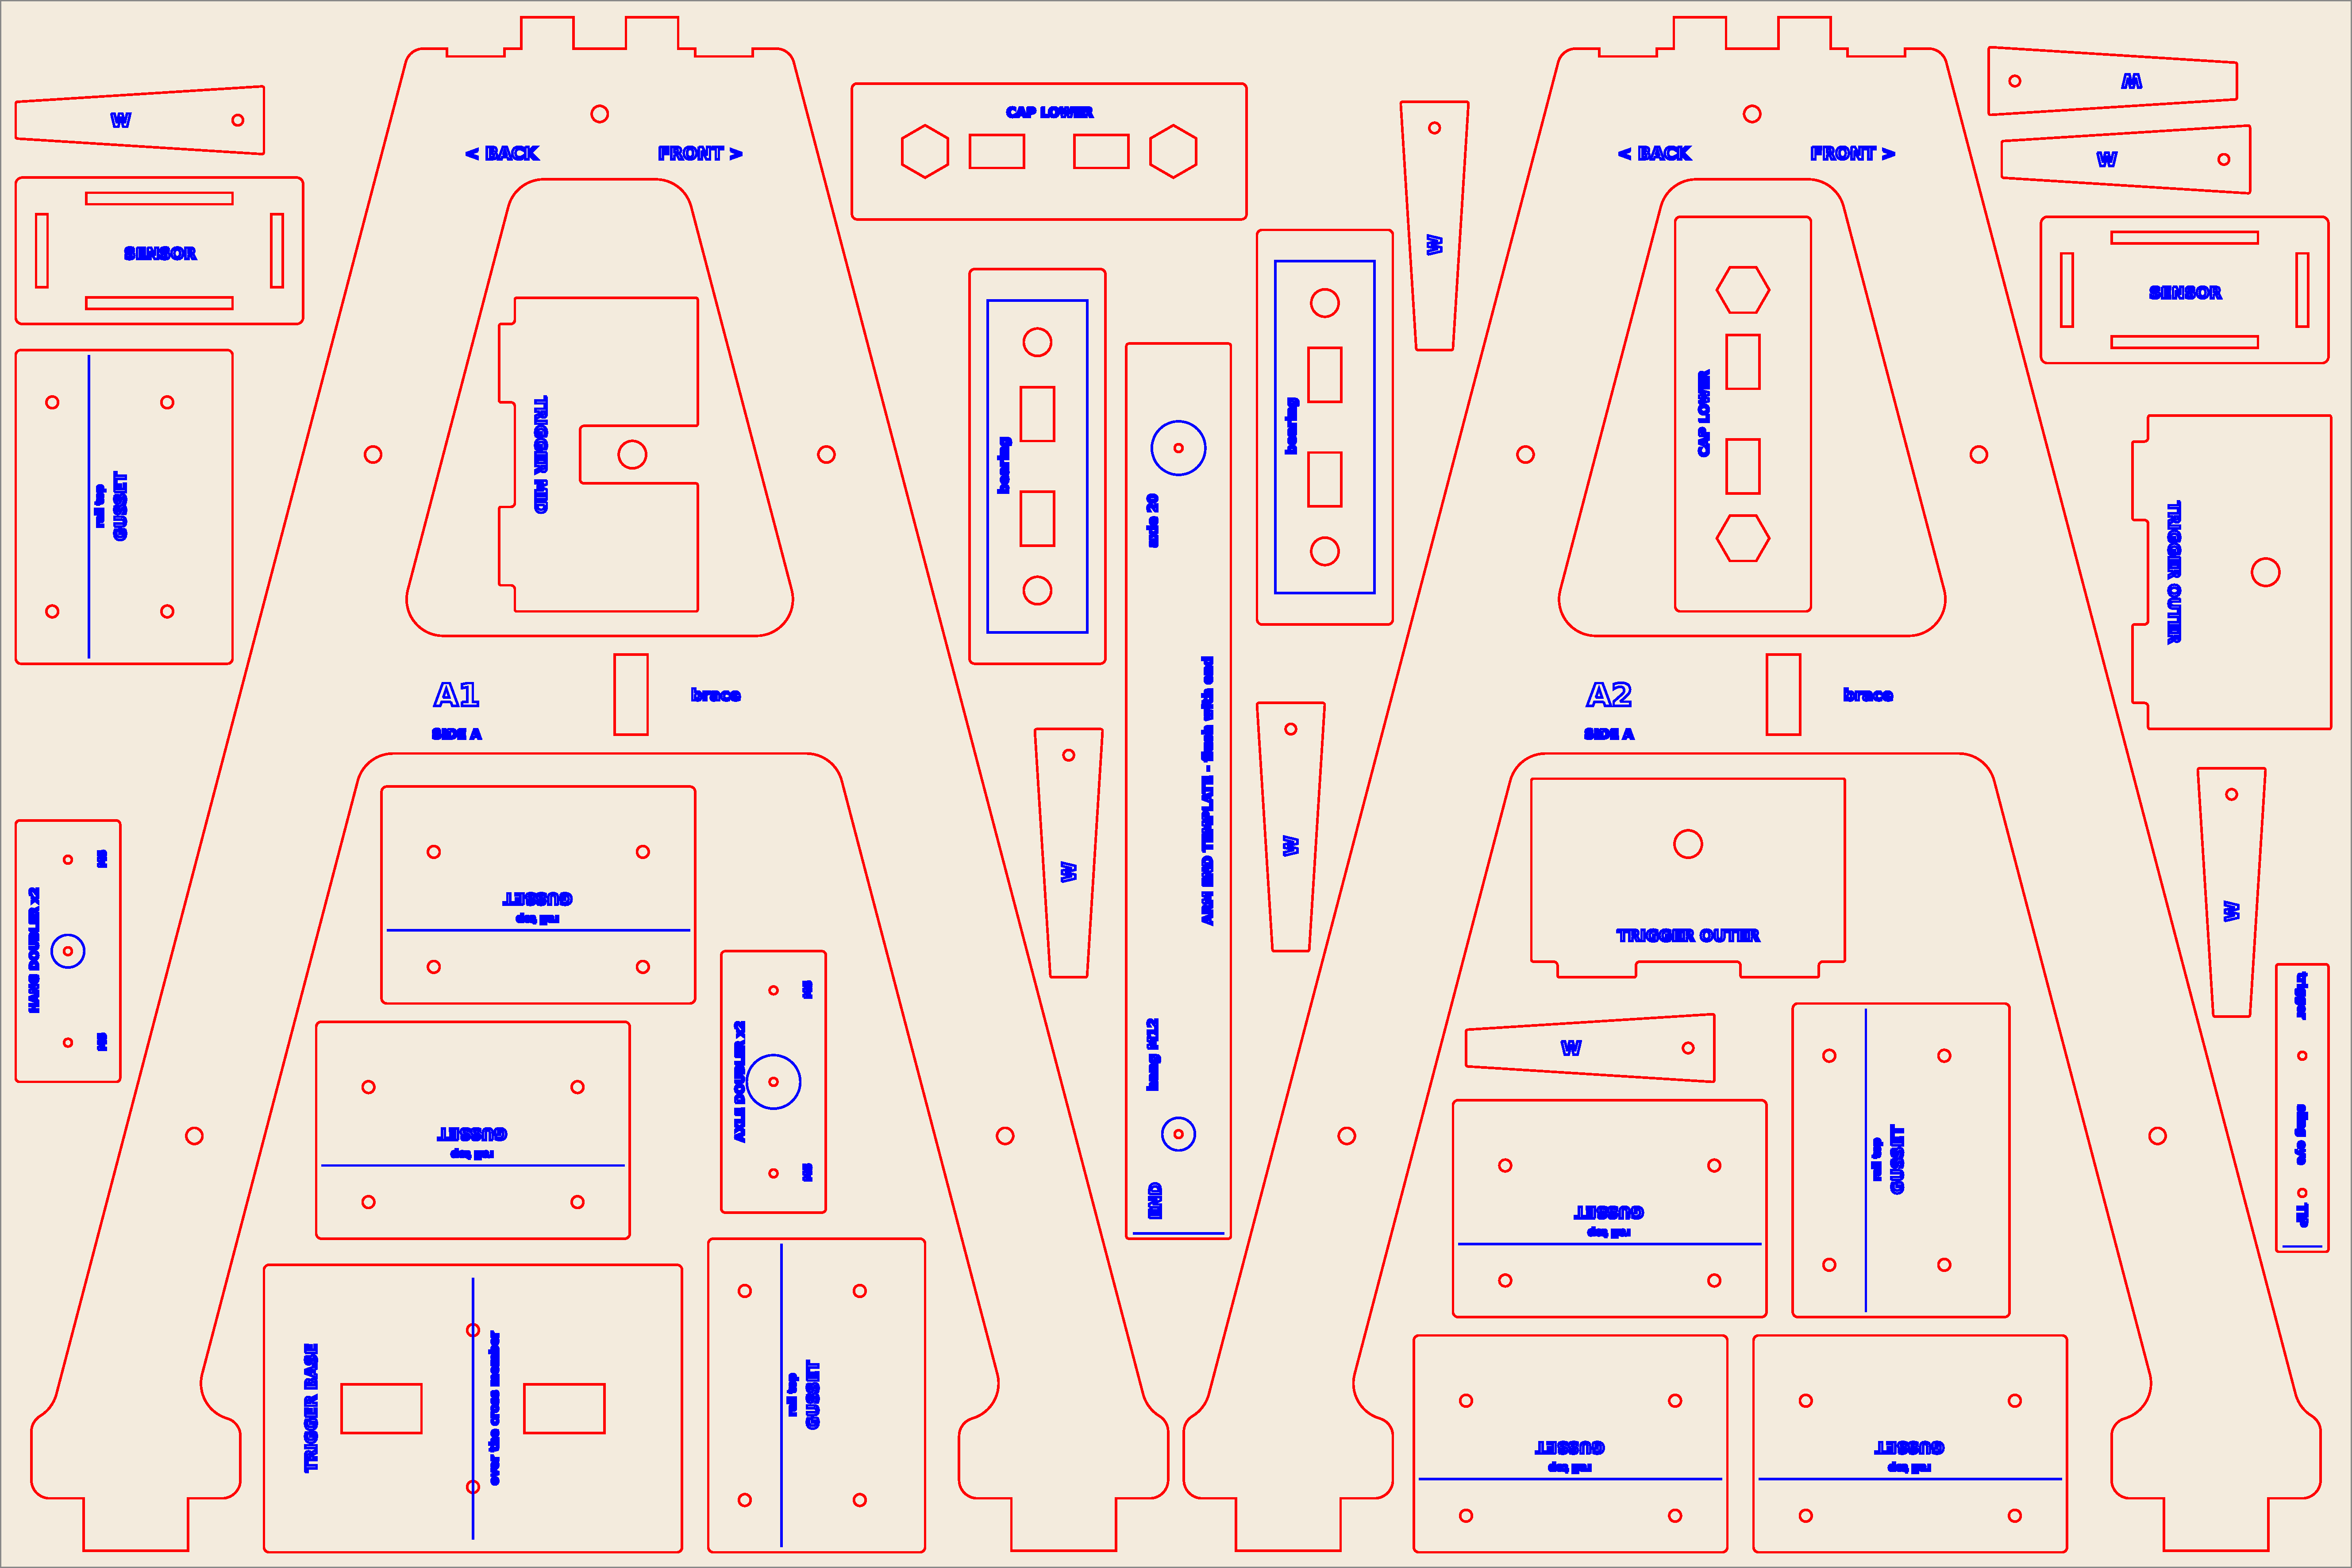
\includegraphics[width=0.40\linewidth]{out/01_Sheet_SIDE_A_panels_preview.pdf}\hspace{4mm}
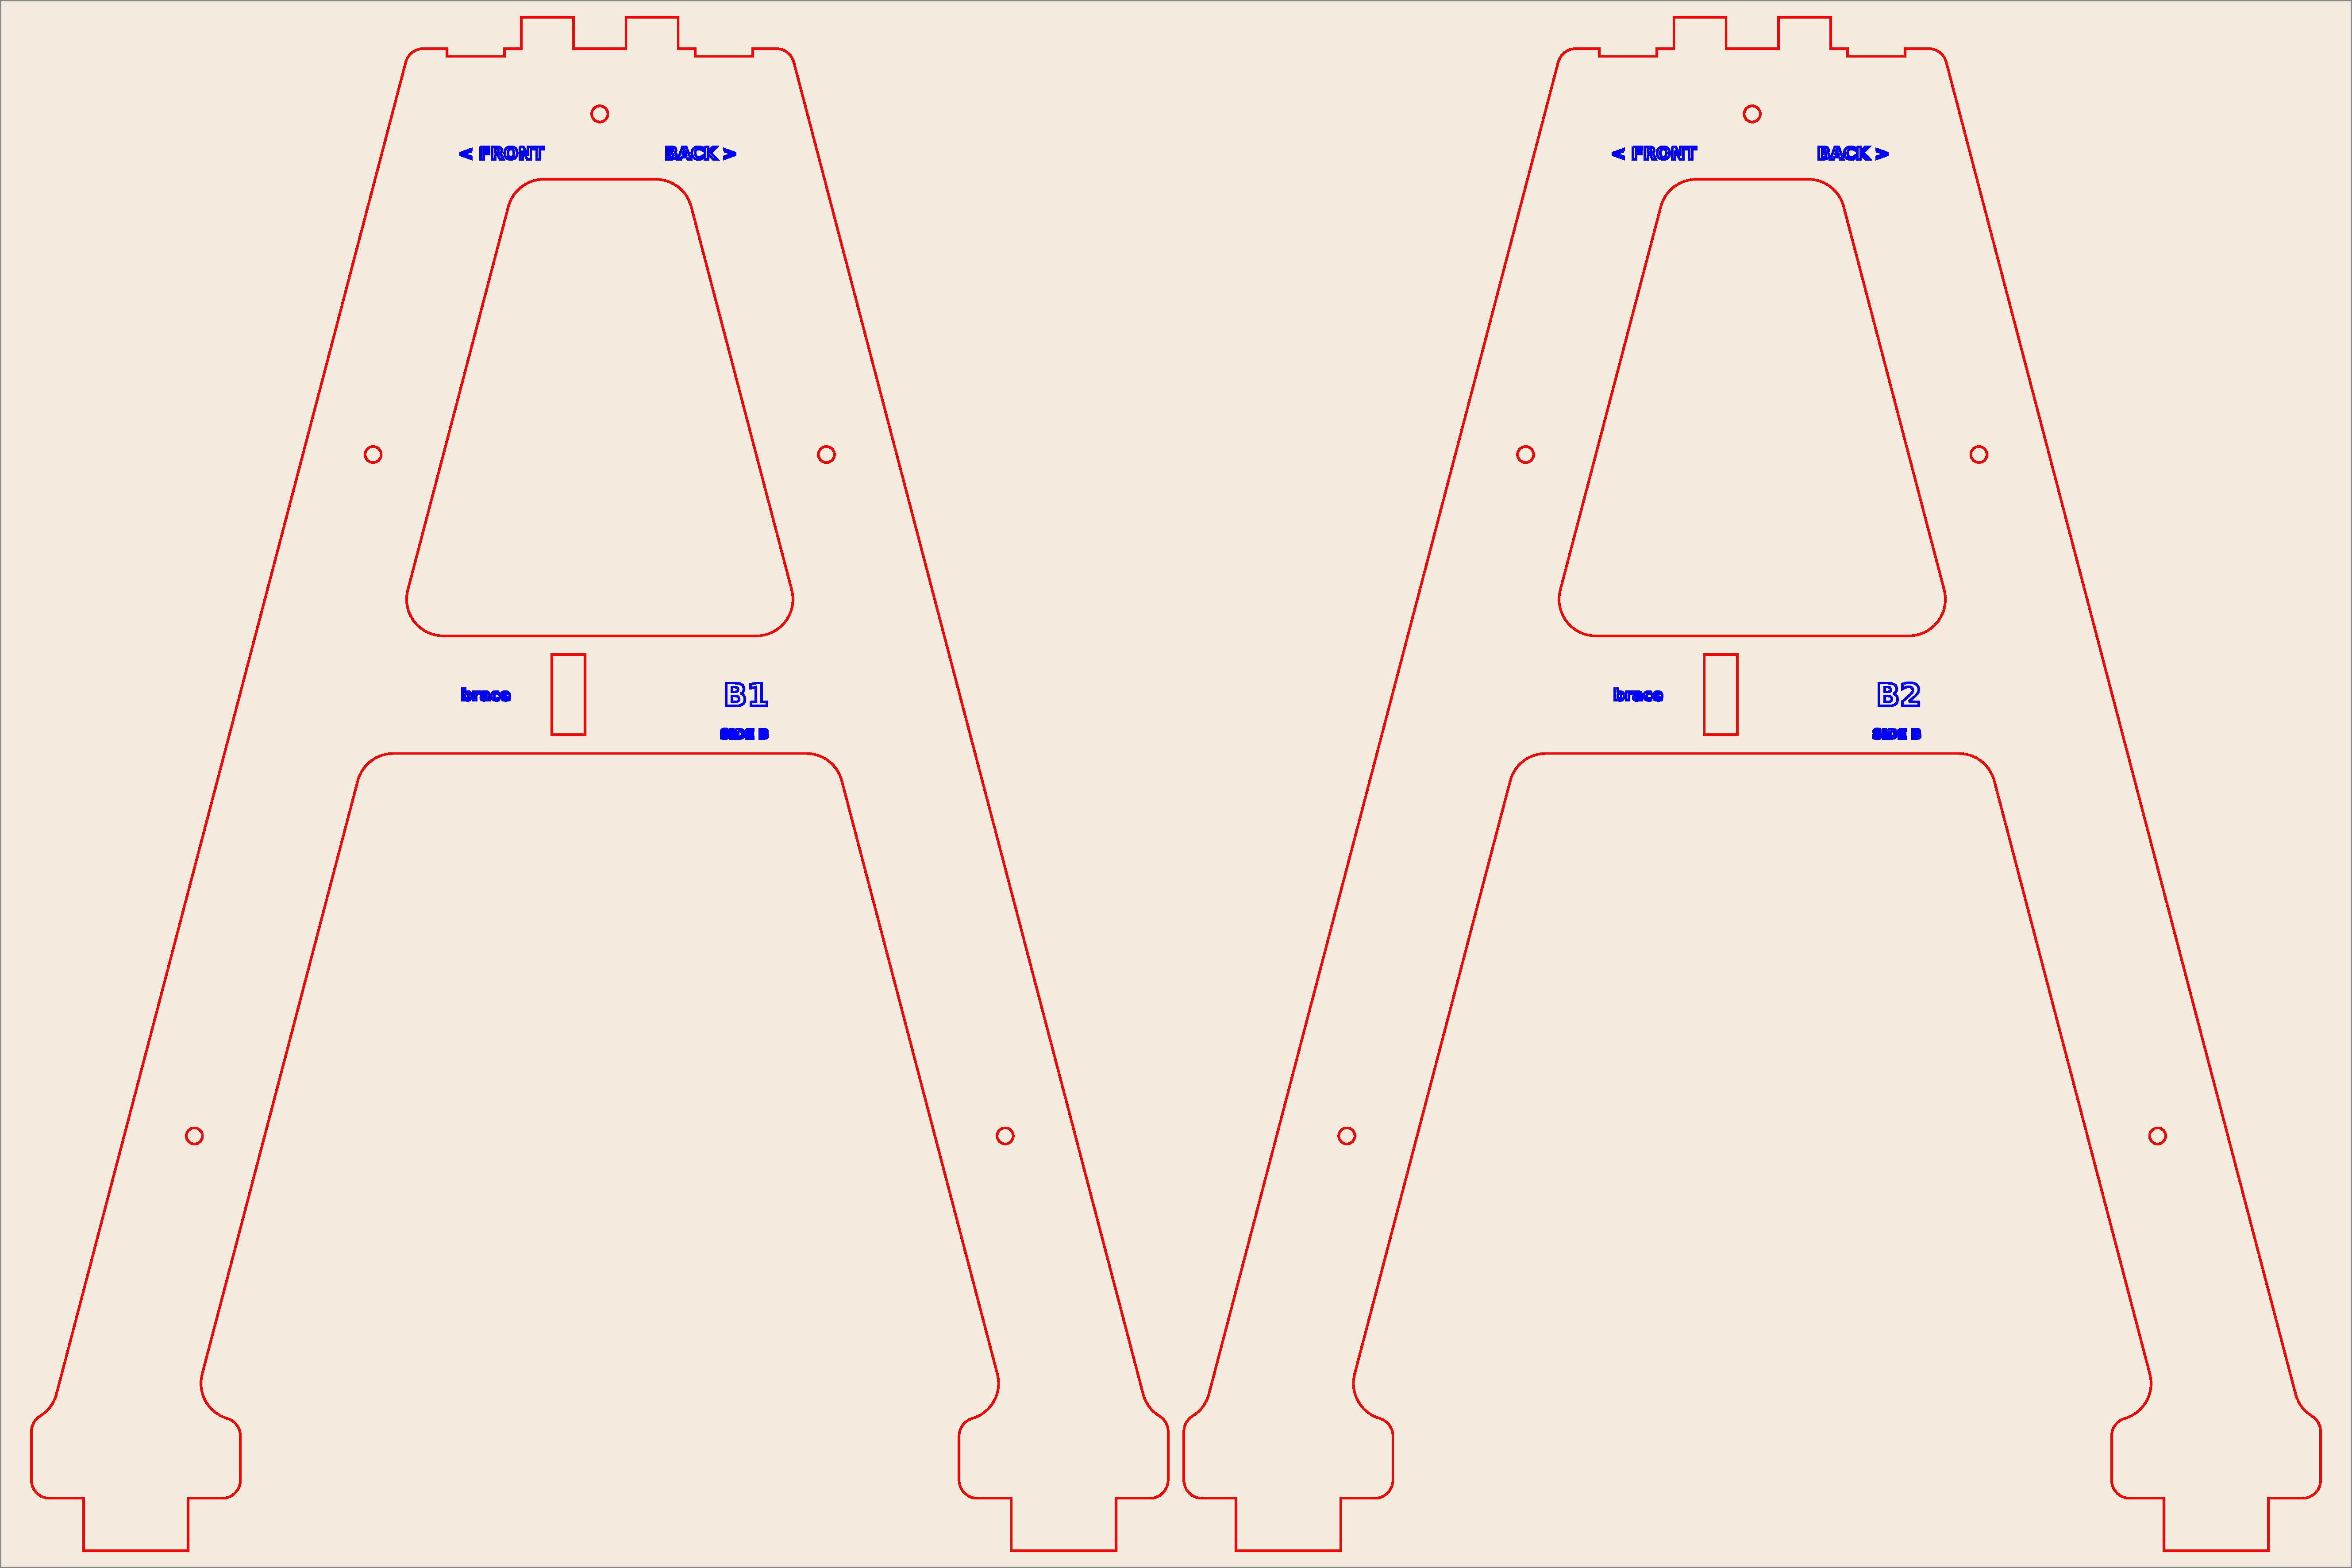
\includegraphics[width=0.40\linewidth]{out/02_Sheet_SIDE_B_panels_preview.pdf}\\[4pt]
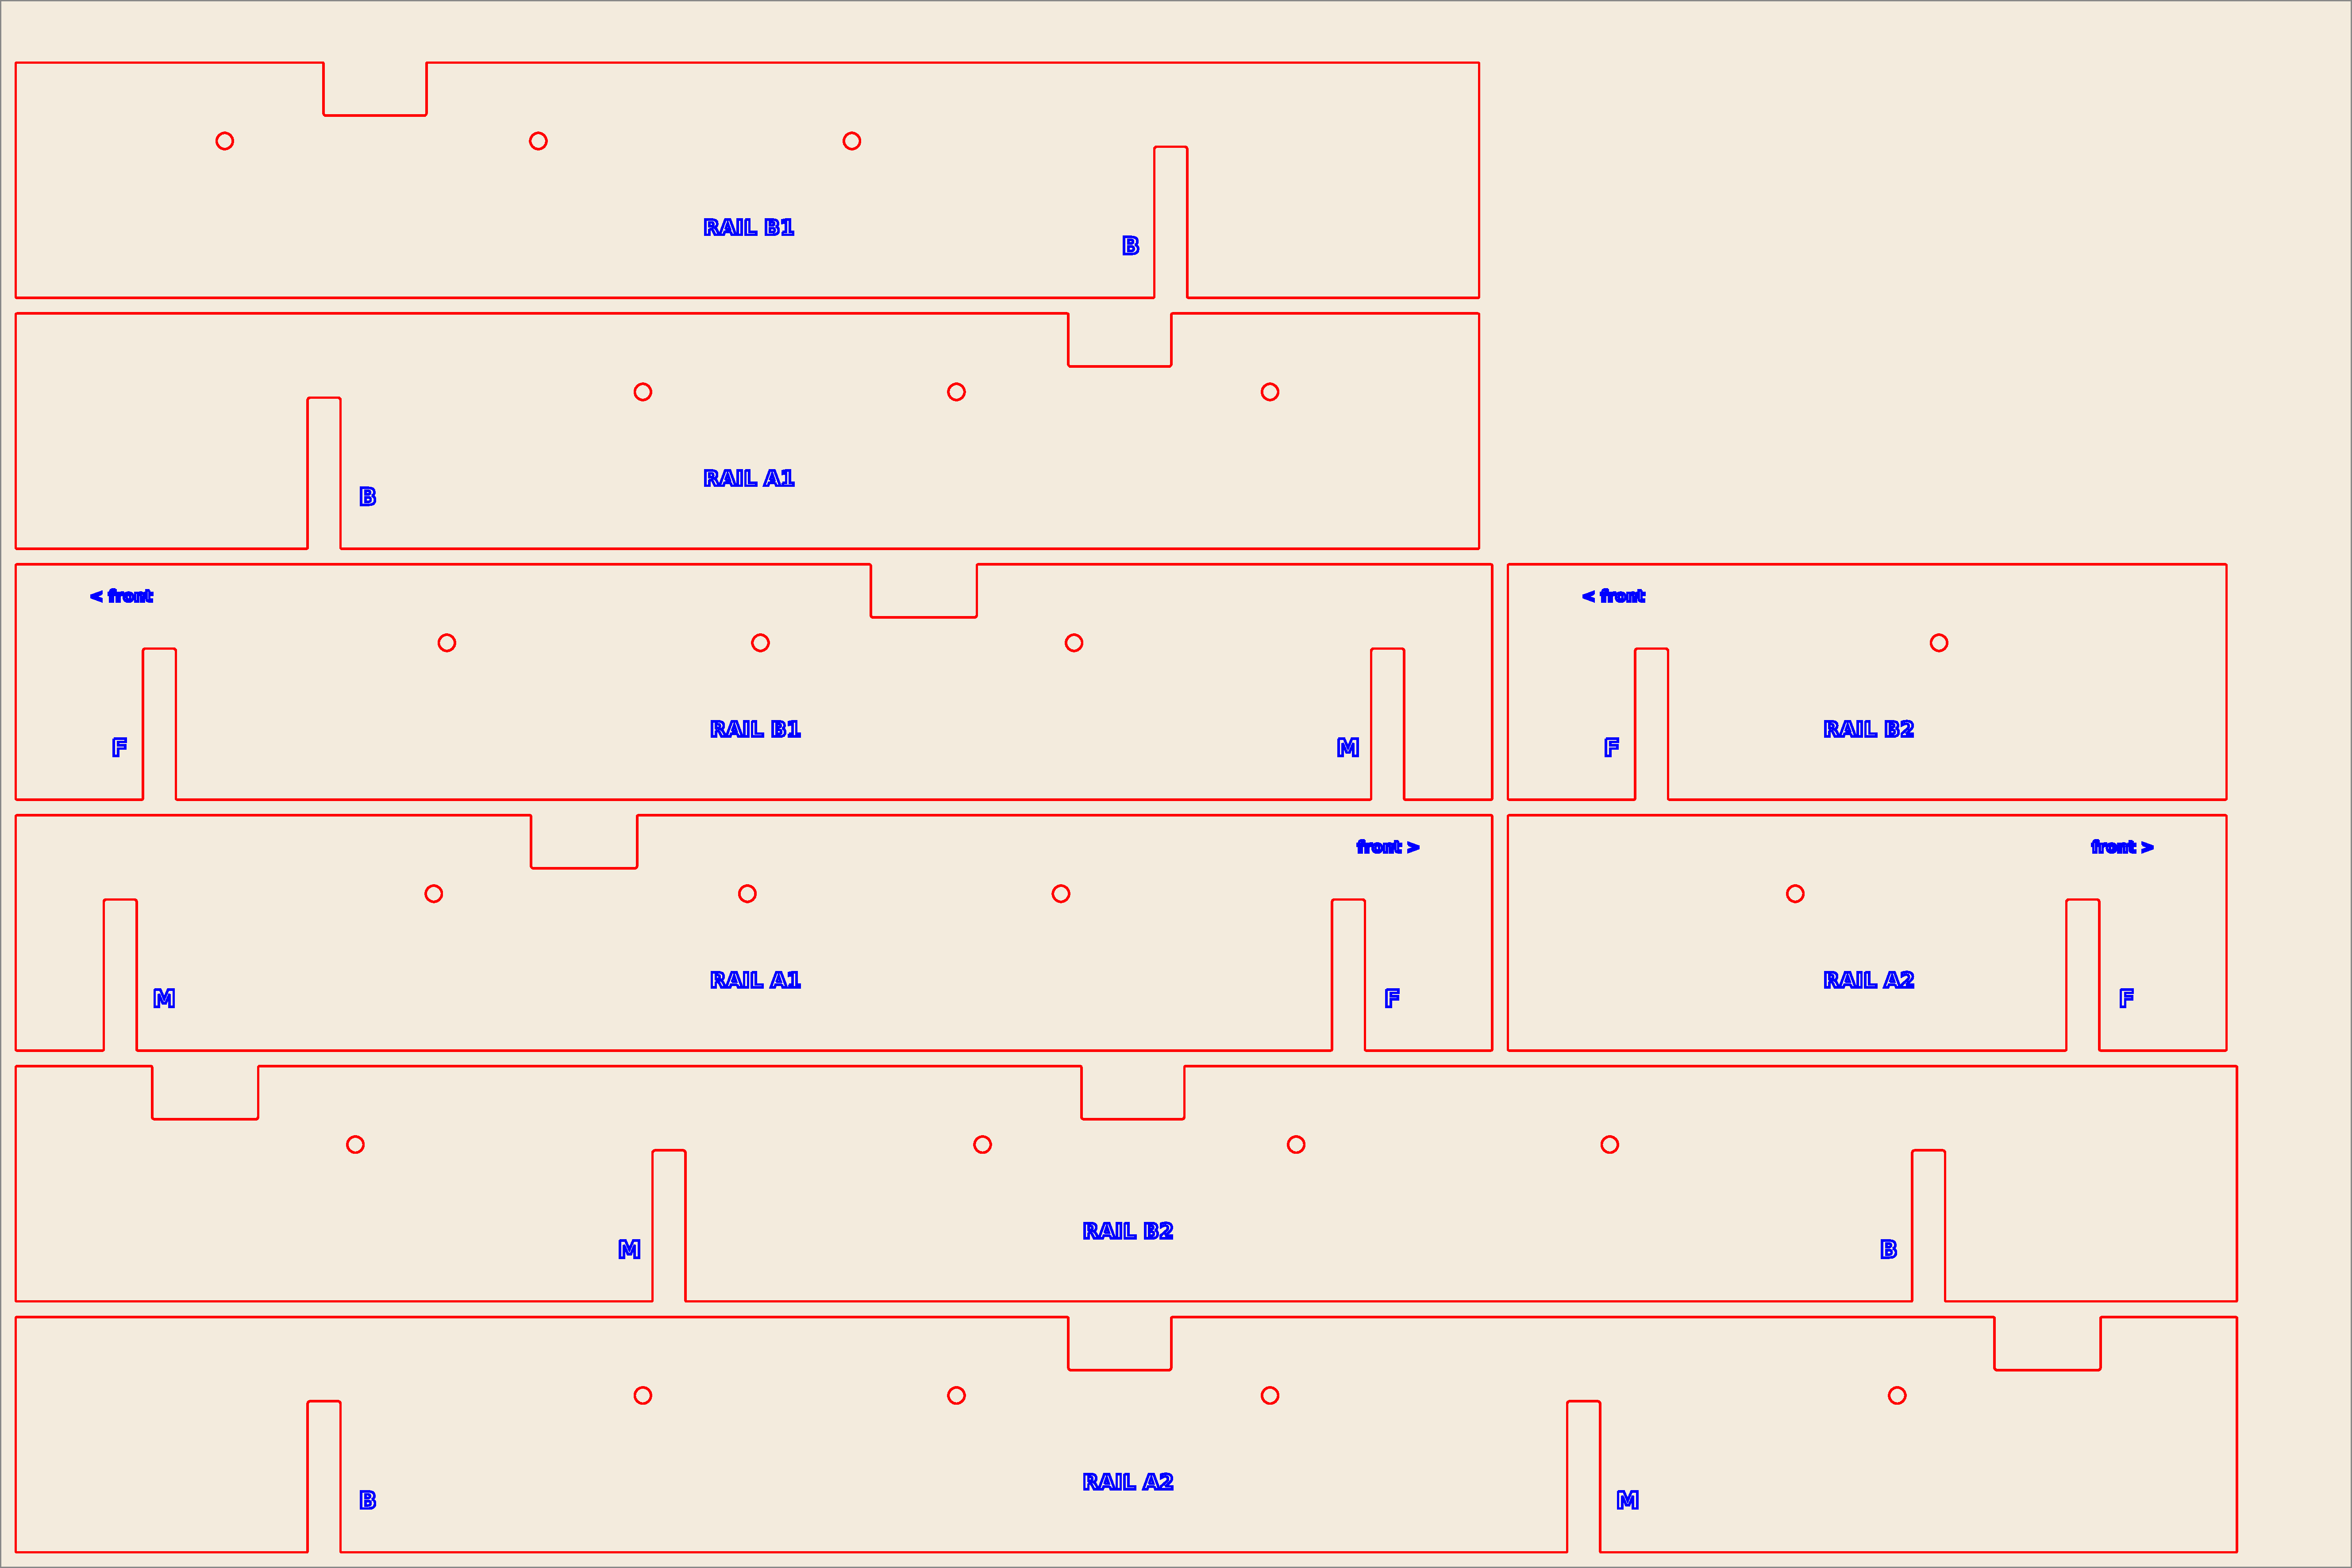
\includegraphics[width=0.40\linewidth]{out/03_Sheet_rails_preview.pdf}\hspace{4mm}
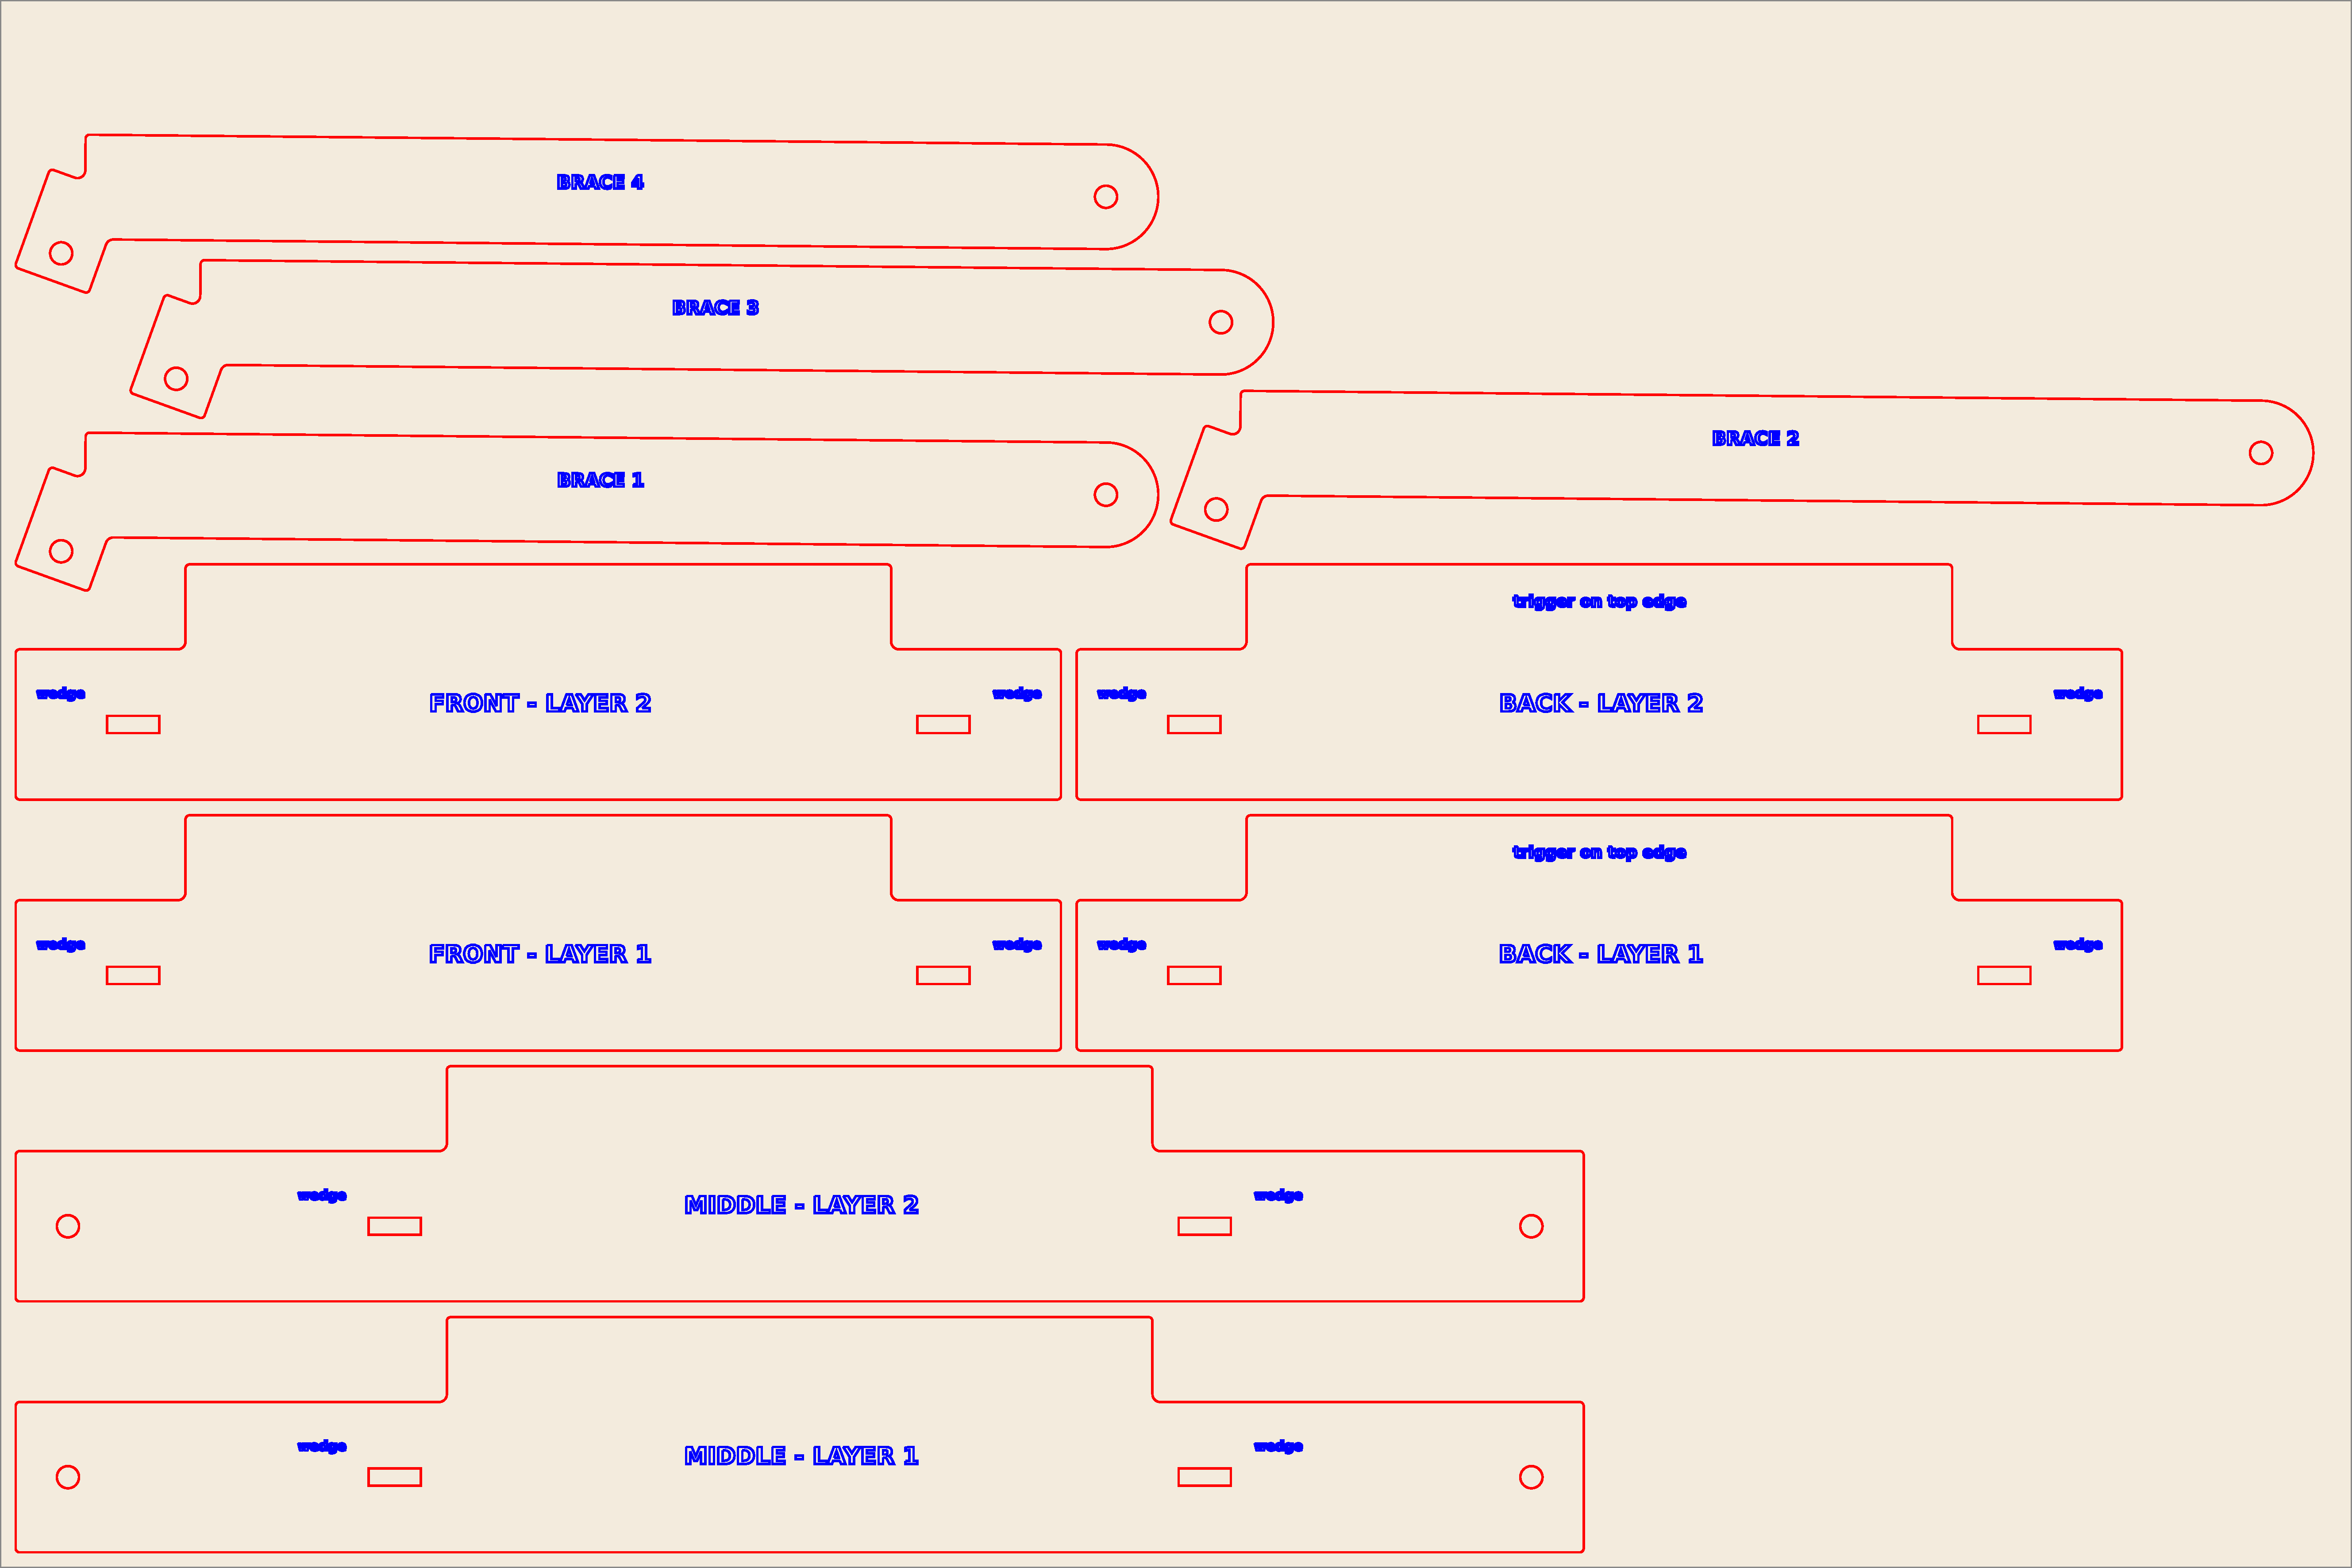
\includegraphics[width=0.40\linewidth]{out/04_Sheet_cross_members_braces_preview.pdf}
\end{center}

\newpage
\sechead{How it goes together}
\begin{center}
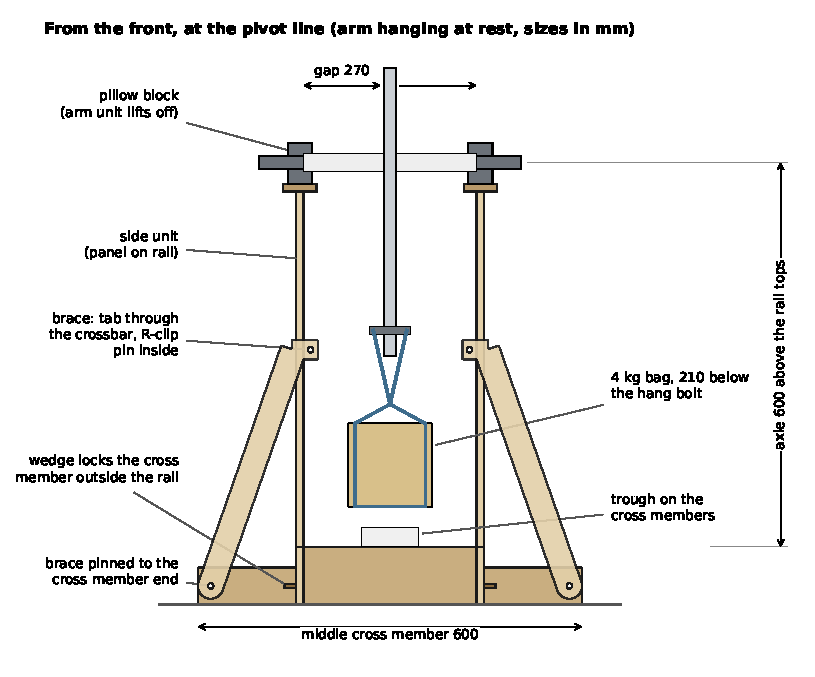
\includegraphics[width=0.58\linewidth]{view_front.pdf}\hfill
\raisebox{3.0cm}{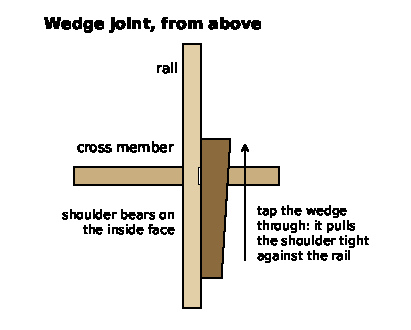
\includegraphics[width=0.36\linewidth]{view_wedge.pdf}}\\[2pt]
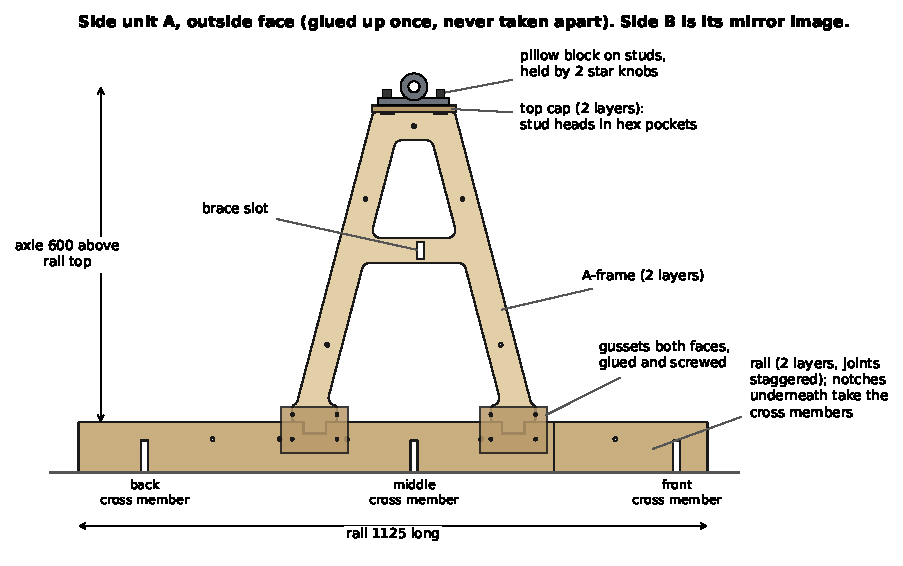
\includegraphics[width=0.74\linewidth]{view_side_unit.pdf}
\end{center}

\sechead{Glue-up (once)}
\begin{minipage}[t]{0.49\linewidth}
\begin{enumerate}[itemsep=1pt, leftmargin=1.5em, topsep=1pt]
  \item \textbf{Keep A and B apart.} Side B is the mirror image of side A. Stack each part's two layers \textbf{as cut, engraving up}, so the engraving ends up on the outside face.
  \item \textbf{A-frames:} PVA between the layers, 6\,mm dowels through the five holes to line them up, clamp flat overnight.
  \item \textbf{Rails:} lay layer 1's two pieces end to end, glue layer 2's two pieces on top (the joints are staggered), dowel and clamp. Check the B, M and F notches line up through both layers.
  \item \textbf{Cross members and braces:} glue each pair (FRONT, MIDDLE, BACK, and braces 1+2, 3+4).
\end{enumerate}
\end{minipage}\hfill
\begin{minipage}[t]{0.49\linewidth}
\begin{enumerate}[itemsep=1pt, leftmargin=1.5em, topsep=1pt, start=5]
  \item \textbf{Side units:} push each A-frame's foot tabs into its rail's top notches; glue and screw a gusset over each foot, on both faces.
  \item \textbf{Top caps:} M10$\times$40 bolts up through the lower cap layer (heads in the hex pockets), glue the upper layer on, then glue the cap over the A-frame's top tabs. The bolts become studs.
  \item \textbf{Trigger:} glue the three trigger layers (slotted one in the middle) into the trigger base, then glue and screw the base along the top edge of the BACK cross member, centred.
  \item \textbf{Arm unit:} drill the arm with the templates, fit the doubler plates, then thread axle, collars, spacers and the two pillow blocks. Fit the sling and the release pin; tune once.
\end{enumerate}
\end{minipage}

\newpage
\sechead{Setting up (two people, about 5 minutes)}
\begin{minipage}[t]{0.49\linewidth}
\textbf{Set up}
\begin{enumerate}[itemsep=1pt, leftmargin=1.5em, topsep=1pt]
  \item Lay the three cross members on the ground: BACK (trigger), MIDDLE (long), FRONT, about where the letters B, M, F are on the rails.
  \item Lower side unit A onto them: each cross member drops into the matching notch under the rail. Repeat with side B. Engraving faces out on both.
  \item Push a wedge through each of the six wedge holes, thin end first, and tap it firm by hand.
  \item Braces: tab through the slot in each crossbar, R-clip pin inside; bottom end pinned to the MIDDLE cross member.
  \item Lift the arm unit on: pillow blocks over the studs, two star knobs each, finger tight plus a quarter turn.
  \item Lay the trough along the cross members; peg or sandbag the base.
  \item Hang the 4\,kg bag (arm at rest, safety strap on). Run the pre-launch checks.
\end{enumerate}
\end{minipage}\hfill
\begin{minipage}[t]{0.48\linewidth}
\textbf{Pack down}: the same steps in reverse.
\begin{enumerate}[itemsep=1pt, leftmargin=1.5em, topsep=1pt]
  \item Bag off first, with the arm at rest.
  \item Star knobs off; lift the arm unit off in one piece and store it flat \textbf{with the sling attached} --- the release pin and sling stay tuned.
  \item Braces off, wedges out, lift the side units off.
\end{enumerate}
\textbf{Store:} 2 side units (about 1125 $\times$ 660\,mm), 3 cross members, 2 braces, the arm unit, and a box with the wedges, pins, R-clips, star knobs, strap cradle, trough, trigger pin and beanbags.

\warnbox{\textbf{Pre-launch checks:} all six wedges tight; four star knobs tight; brace pins and R-clips in; the arm swings a full turn by hand without touching anything; the bag clears the trough at the bottom of its swing; base pegged or sandbagged.}
\end{minipage}

\sechead{Sizes and expected range}
\begin{minipage}[t]{0.49\linewidth}
{\footnotesize
\begin{tabularx}{\linewidth}{@{}Y r@{}}
\toprule
Throwing arm (axle to release pin) & 750 \\
Short arm (axle to hang bolt) & 262.5 \\
Bag hang (bolt to bag centre) & 210 \\
Sling (tip to pouch centre) & 750 \\
Axle above rail tops & 600 \\
Gap between the sides & 270 \\
Rails & 1125 \\
Cross members: middle / front, back & 600 / 400 \\
Aluminium arm tube & 1055 \\
\bottomrule
\end{tabularx}}
\end{minipage}\hfill
\begin{minipage}[t]{0.48\linewidth}
{\footnotesize
\begin{tabularx}{\linewidth}{@{}Y c c@{}}
\toprule
\textbf{Beanbag (4\,kg sand)} & \textbf{Plan on} & \textbf{Best case} \\
\midrule
25\,g & 23\,m & 33\,m \\
50\,g & 20\,m & 28\,m \\
75\,g & 16\,m & 23\,m \\
100\,g & 13\,m & 19\,m \\
125\,g & 10\,m & 15\,m \\
\bottomrule
\end{tabularx}}

{\footnotesize From the computer model; ``plan on'' is 30\,\% less for real-world losses. Peak arm spin about 9--15\,rad/s.}
\end{minipage}

\sechead{Also needed}
{\footnotesize
\begin{tabularx}{\linewidth}{@{}Y L{1.3cm} Y L{1.3cm}@{}}
\toprule
\textbf{Item} & \textbf{Qty} & \textbf{Item} & \textbf{Qty} \\
\midrule
6\,mm plywood, 900$\times$600 & 4 sheets & 8\,mm clevis pins + R-clips (braces) & 4 \\
UCP204 pillow blocks (20\,mm bore) & 2 & 10\,mm trigger pin, 60 long & 1 \\
M10$\times$40 hex bolts (studs) + M10 star knobs & 4 + 4 & 6\,mm dowel, 30 long & 20 \\
20\,mm steel axle, 360 long; 2 shaft collars & 1 & 25\,mm wood screws (gussets, trigger base) & 40 \\
Spacer tubes (25\,mm conduit), 112 long & 2 & Aluminium tube 40$\times$20$\times$1.6, 1055 long & 1 \\
M12$\times$50 hang bolt, nyloc nut, washers & 1 & 6\,mm aluminium plate 100$\times$40 (doublers) & 4 \\
M6 eye bolts (sling eye, trigger eye) & 2 & M5$\times$40 bolts for the doublers & 6 \\
Rated strap cradle and shackle & 1 & 90\,mm PVC pipe, halved, 900 long (trough) & 1 \\
\bottomrule
\end{tabularx}}

\end{document}
